\documentclass[12pt, letterpaper]{article}
\usepackage[utf8]{inputenc}
\usepackage[spanish]{babel}
\usepackage{graphicx}

\title{Tarea 2}
\author{Hiram Isaí Torres Espinosa}
\date{\today}

\begin{document}

    \begin{titlepage}
        \maketitle
    \end{titlepage}


    \begin{abstract}
        \begin{itemize}
            \item El Primero punto resuelve la duda sobre como es el funcionamiento de una máquina de vapor, explicado brevemente.  
            \item El segundo explica a través de un diagrama la ubicación y el nombre de cada parte de la máquina de vapor. 
        \end{itemize}
        
    \end{abstract}


    \section{Explicación}
        La máquina de vapor está catalogada como un motor de combustión externa, su función es el de transformar agua a vapor de agua para luego ser utilizado como energía mecánica.
        \\ El funcionamiento de la máquina de vapor esta dividido en tres principales partes: \\
        \begin{enumerate}
            \item El sistema tiene una caldera cerrada hermeticamente la cual se calienta, por medio de la quema de algun combistible para generar el vapor de agua directamente.
            \item El vapor es introducido a presión dentro del cilindro, haciendo que este produzca el movimiento lineal del pintón o émbolo, este hace que por medio del sistema biela-manivela, haga un movimiento circular y poder dar paso a la energía mecánica utilizada en distintas industrias. 
            \item El control de la potencia para esta máquina es importante, y un sistema ideado para esto, es utilizando válvulas que regulan el flujo del vapor a través del sistema, evitando así el exceso de presión en la máquina.  
        \end{enumerate}
        y así es de forma breve la explicación de como funciona una máquina de vapor. 
       
    
    \begin{figure}
        \section{Diagrama}
        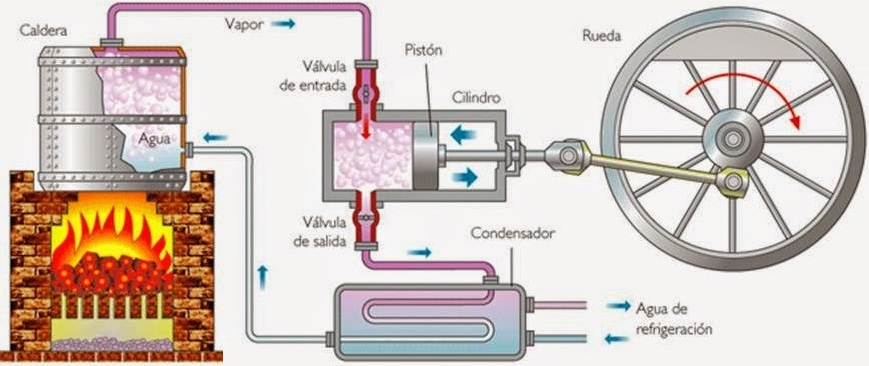
\includegraphics[scale=0.75]{steammachine.jpg}
        \caption{Partes de la máquina de vapor} 

        
            
    
    
       
    \end{figure}
        
    
    
    
\end{document}